\documentclass[12pt]{article}
% =========================================================================
% Coal-Plant Pollution Controls and Infant Health in Texas
% Sayorn Chin (Lafayette College)
% STATUS: scaffold. Empirical sections drafted from the analysis pipeline;
% Intro/Conclusion are structured drafts for the author to refine in his voice.
% Compile: xelatex -> bibtex -> xelatex x2  (BIBINPUTS=..)
% =========================================================================
\usepackage[margin=1in]{geometry}
\usepackage{amsmath,amssymb}
\usepackage{booktabs}
\usepackage{graphicx}
\graphicspath{{figures/}}
\usepackage[round]{natbib}
\usepackage{setspace}
\usepackage[hidelinks]{hyperref}
\usepackage{caption}
\onehalfspacing

\title{\textbf{Do Coal-Plant Pollution Controls Improve Infant Health?\\
Evidence from CAIR-Era Retrofits in Texas}}
\author{Sayorn Chin\thanks{Department of Economics, Lafayette College, Easton, PA.
Confidential Texas vital-records microdata used under data-use agreement; analysis
code is available, data are not redistributed.}}
\date{June 2026 --- \emph{Preliminary draft}}

\begin{document}
\maketitle

\begin{abstract}
\noindent We ask whether the wave of pollution-control retrofits at U.S.\ coal-fired
power plants---scrubbers, selective catalytic reduction, baghouses, and activated-carbon
injection installed largely under the Clean Air Interstate Rule (CAIR)---delivered
measurable infant-health co-benefits. Using confidential, census-tract-geocoded Texas
birth and fetal-death records (2005--2010), staggered retrofit dates from EIA-860, and
unit-level continuous-emissions monitoring (CEMS), we trace the full causal chain from
retrofit to plant emissions to local ambient pollution to health at birth. The first link
is strong and directly verified: retrofits sharply reduce plant SO$_2$/NO$_x$ emissions at
their installation dates. The chain breaks at the second link: within tract and time fixed
effects, coal-plant emissions exposure does \emph{not} move local ambient PM$_{2.5}$
(first-stage $F=0.25$) or SO$_2$ ($p=0.97$), with only a weak, fragile signal for lead.
Consistent with this, we find no coal-attributable effect on birth weight, low birth weight,
or fetal death; general ambient PM$_{2.5}$ is associated with the low-birth-weight tail and
fetal death only at borderline significance. We interpret the precisely-estimated null as
evidence that coal plants' marginal contribution to \emph{local population} ambient exposure
in this setting was too small to generate detectable infant-health co-benefits---coal
SO$_2$/NO$_x$ become regional secondary particulates rather than local primary exposure.
The result bounds the local infant-health co-benefits of coal-plant control retrofits and
clarifies where such co-benefits should and should not be sought.
\end{abstract}

\section{Introduction}
% [DRAFT — author to set framing/voice. Verified anchors cited below.]
The health co-benefits of air-quality regulation are a central input to cost--benefit
analysis of environmental policy. A large literature links air pollution to infant health,
typically finding the clearest effects on infant mortality and the tails of the birth-outcome
distribution \citep{chay2003air,currie2009air,currie2011traffic,knittel2016caution}. Whether
\emph{cleaning up} coal-fired power plants---the largest stationary source of SO$_2$ and
NO$_x$---improves infant health is less settled; the closest precedent,
\citet{luechinger2014air}, finds that mandated desulfurization in Germany reduced infant
mortality, though not uniformly on birth weight.

% TODO(author): position contribution; (1) U.S. CEMS-verified retrofit design;
% (2) full chain retrofit->emissions->ambient->health; (3) tract-geocoded vital records.
This paper studies the CAIR-era retrofit wave at Texas coal plants and asks the
intent-to-treat question directly: did installing controls improve infant health nearby?

\section{Setting: Coal Plants and CAIR-Era Retrofits in Texas}
% [DRAFT] Texas is the largest U.S. coal-power state. Under CAIR (2005) and related
% programs, 12 Texas coal plants installed major emission controls in 2003--2010
% (concentrated 2008--2010): FGD scrubbers, SCR/SNCR, baghouses, activated-carbon injection.
% Treatment timing is staggered and driven by federal/state compliance schedules.

\section{Data}
\textbf{Births and fetal deaths.} Confidential Texas vital records, geocoded to census-tract
centroid. The usable window is 2005--2010 (earlier years are incompletely populated). Primary
outcome: birth weight; secondary: low birth weight ($<2{,}500$g) and the fetal-death rate.\\
\textbf{Retrofits.} EIA-860 Schedule 6 (emissions-control equipment) gives the control type and
in-service date for each plant.\\
\textbf{Emissions.} EPA CEMS daily unit-level SO$_2$/NO$_x$ confirm the emission change at each
retrofit.\\
\textbf{Ambient pollution.} EPA AQS monitors for PM$_{2.5}$, SO$_2$, and lead. Exposure is the
pregnancy-window (trailing nine-month) ambient mean at the nearest monitor.

\section{Empirical Strategy}
We decompose the policy question into three links: (1) retrofit $\to$ plant emissions; (2) plant
emissions $\to$ local ambient pollution; (3) ambient pollution $\to$ infant health. For (2)--(3)
we estimate, at the birth level,
\[
y_{i t} = \beta\, \text{Exposure}_{c(i),t} + \alpha_{c(i)} + \delta_t + \varepsilon_{it},
\]
with census-tract ($\alpha_c$) and birth-year-month ($\delta_t$) fixed effects and standard
errors clustered by monitor. Coal-attributable exposure is inverse-distance-weighted CEMS
emissions; we also instrument ambient pollution with coal-emissions exposure (2SLS) and report a
staggered-adoption event study (Callaway--Sant'Anna) of the retrofit itself in the proximity sample.

\section{Results}
\textbf{Link 1 (strong).} CEMS shows sharp emission reductions at retrofit dates---e.g.\ W.A.\
Parish NO$_x$ falls from $\sim$1{,}000 to $\sim$350 tons/month at its 2004 SCR installation, and
Pirkey's SO$_2$ falls $\sim$85\% at its 2006 control (Figure~\ref{fig:firststage}).

\textbf{Link 2 (broken).} Within tract and time fixed effects, coal-emissions exposure does not
predict local ambient pollution: the first-stage coefficient is small and insignificant for
PM$_{2.5}$ ($F=0.25$) and SO$_2$ ($p=0.97$), with only a weak, fragile lead signal
(Table~\ref{tab:results_main}, Panel B).

\textbf{Link 3 (null/borderline).} There is no coal-attributable effect on birth weight or low
birth weight (Panel D). General ambient PM$_{2.5}$ is associated with the low-birth-weight tail
($p=0.065$) and the fetal-death rate ($p=0.10$) only at borderline significance, and mean birth
weight is a precise null; the SO$_2$/lead health coefficients are wrong-signed and reflect
confounding/small-cluster artifacts (Panel C).

\begin{table}[htbp]
\centering
\caption{The causal chain: coal-plant control retrofits $\to$ emissions $\to$ ambient pollution $\to$ infant health, Texas 2005--2010}
\label{tab:results_main}
\small
\begin{tabular}{lccc}
\toprule
 & PM$_{2.5}$ & SO$_2$ & Lead \\
\midrule
\multicolumn{4}{l}{\textit{Panel A. Link 1: retrofit $\to$ plant emissions (EPA CEMS)}} \\
\quad Emission drop at retrofit & \multicolumn{3}{c}{Strong; verified (e.g.\ W.A.\ Parish NO$_x$ $\downarrow$ at 2004 SCR; Pirkey SO$_2$ $-85\%$ at 2006)} \\[4pt]
\multicolumn{4}{l}{\textit{Panel B. Link 2: coal-emissions exposure $\to$ local ambient (per SD; tract$+$ym FE)}} \\
\quad Ambient level & 0.67 & 0.017 & 0.0008 \\
\quad \quad (SE) & (1.32) & (0.51) & (0.0004) \\
\quad First-stage $F$ & 0.25 & 0.00 & 4.6 \\[4pt]
\multicolumn{4}{l}{\textit{Panel C. Link 3: ambient pollution $\to$ infant health (per unit; tract$+$ym FE)}} \\
\quad Birth weight (g) & $-0.83$ & $2.74^{**}$ & 4.0 \\
\quad \quad (SE) & (1.46) & (1.05) & (492) \\
\quad Low birth weight (pp) & $0.083^{*}$ & $-0.095^{*}$ & $-0.35^{***}$ \\
\quad \quad (SE) & (0.044) & (0.053) & (0.104) \\
\quad Fetal-death rate (per 1{,}000) & $0.19$ & --- & --- \\
\quad \quad (SE) & (0.11) & & \\[4pt]
\multicolumn{4}{l}{\textit{Panel D. Reduced form: coal-emissions exposure $\to$ health (per SD)}} \\
\quad Birth weight (g) & \multicolumn{3}{c}{$6.3$ \ (5.1), $p=0.22$} \\
\quad Low birth weight (pp) & \multicolumn{3}{c}{$-0.22$ \ (0.16), $p=0.19$} \\
\midrule
\multicolumn{4}{p{0.92\linewidth}}{\footnotesize \textit{Notes.} Births within 30 km of an ambient monitor (PM$_{2.5}$/SO$_2$/lead) and 50 km of a coal plant, Texas 2005--2010; confidential tract-geocoded vital records. All specifications include census-tract and birth-year-month fixed effects; standard errors clustered by monitor. Exposure is the pregnancy-window (trailing 9-month) ambient mean at the nearest monitor; coal-emissions exposure is inverse-distance-weighted CEMS SO$_2$+NO$_x$. Lead estimates rest on 10 monitor clusters. $^{*}p<0.10$, $^{**}p<0.05$, $^{***}p<0.01$. The wrong-signed SO$_2$/lead health coefficients reflect confounding/small-cluster artifacts, not protective effects; see text.} \\
\bottomrule
\end{tabular}
\end{table}


\begin{figure}[htbp]
\centering
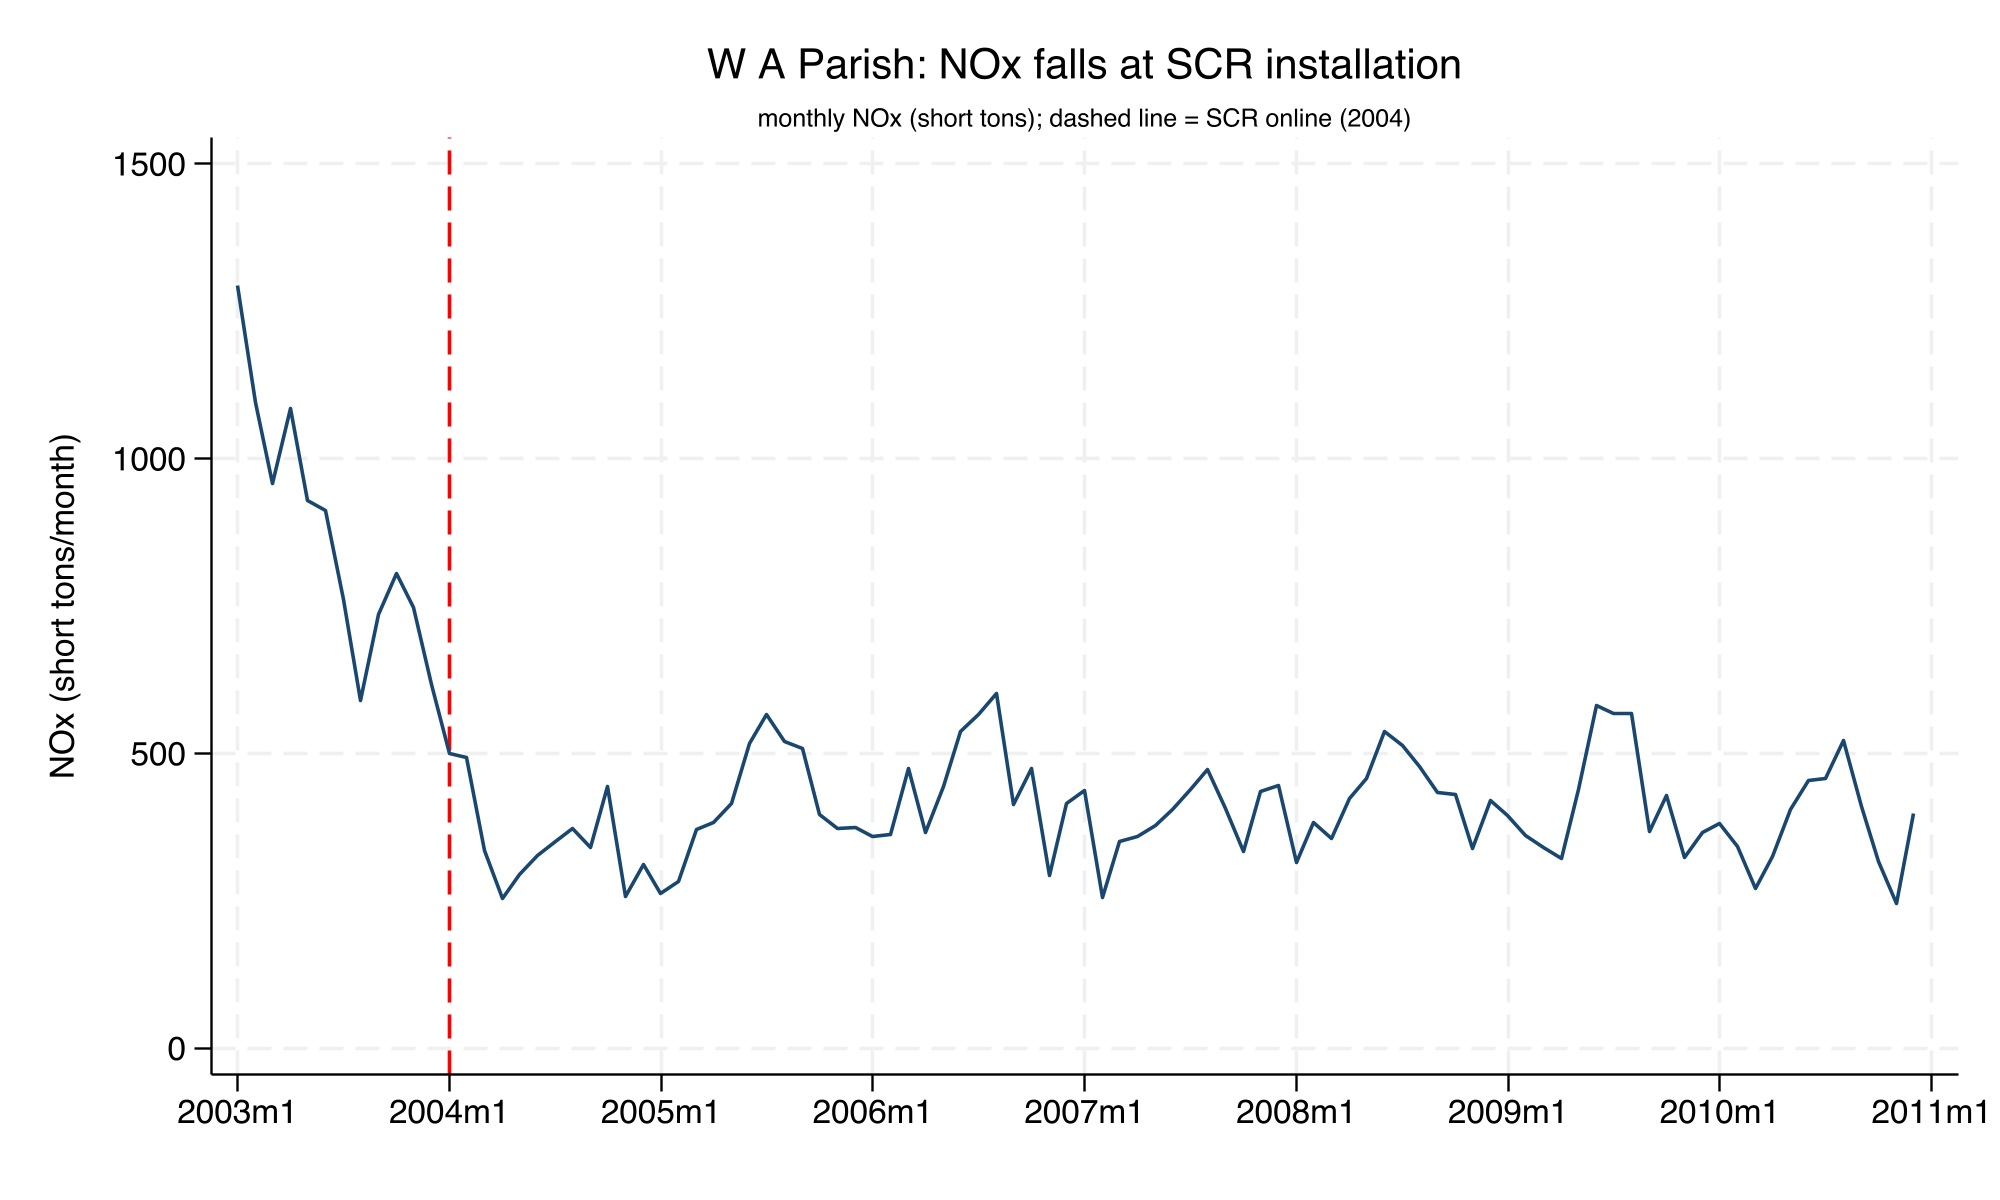
\includegraphics[width=0.49\linewidth]{hero_parish_nox.png}\hfill
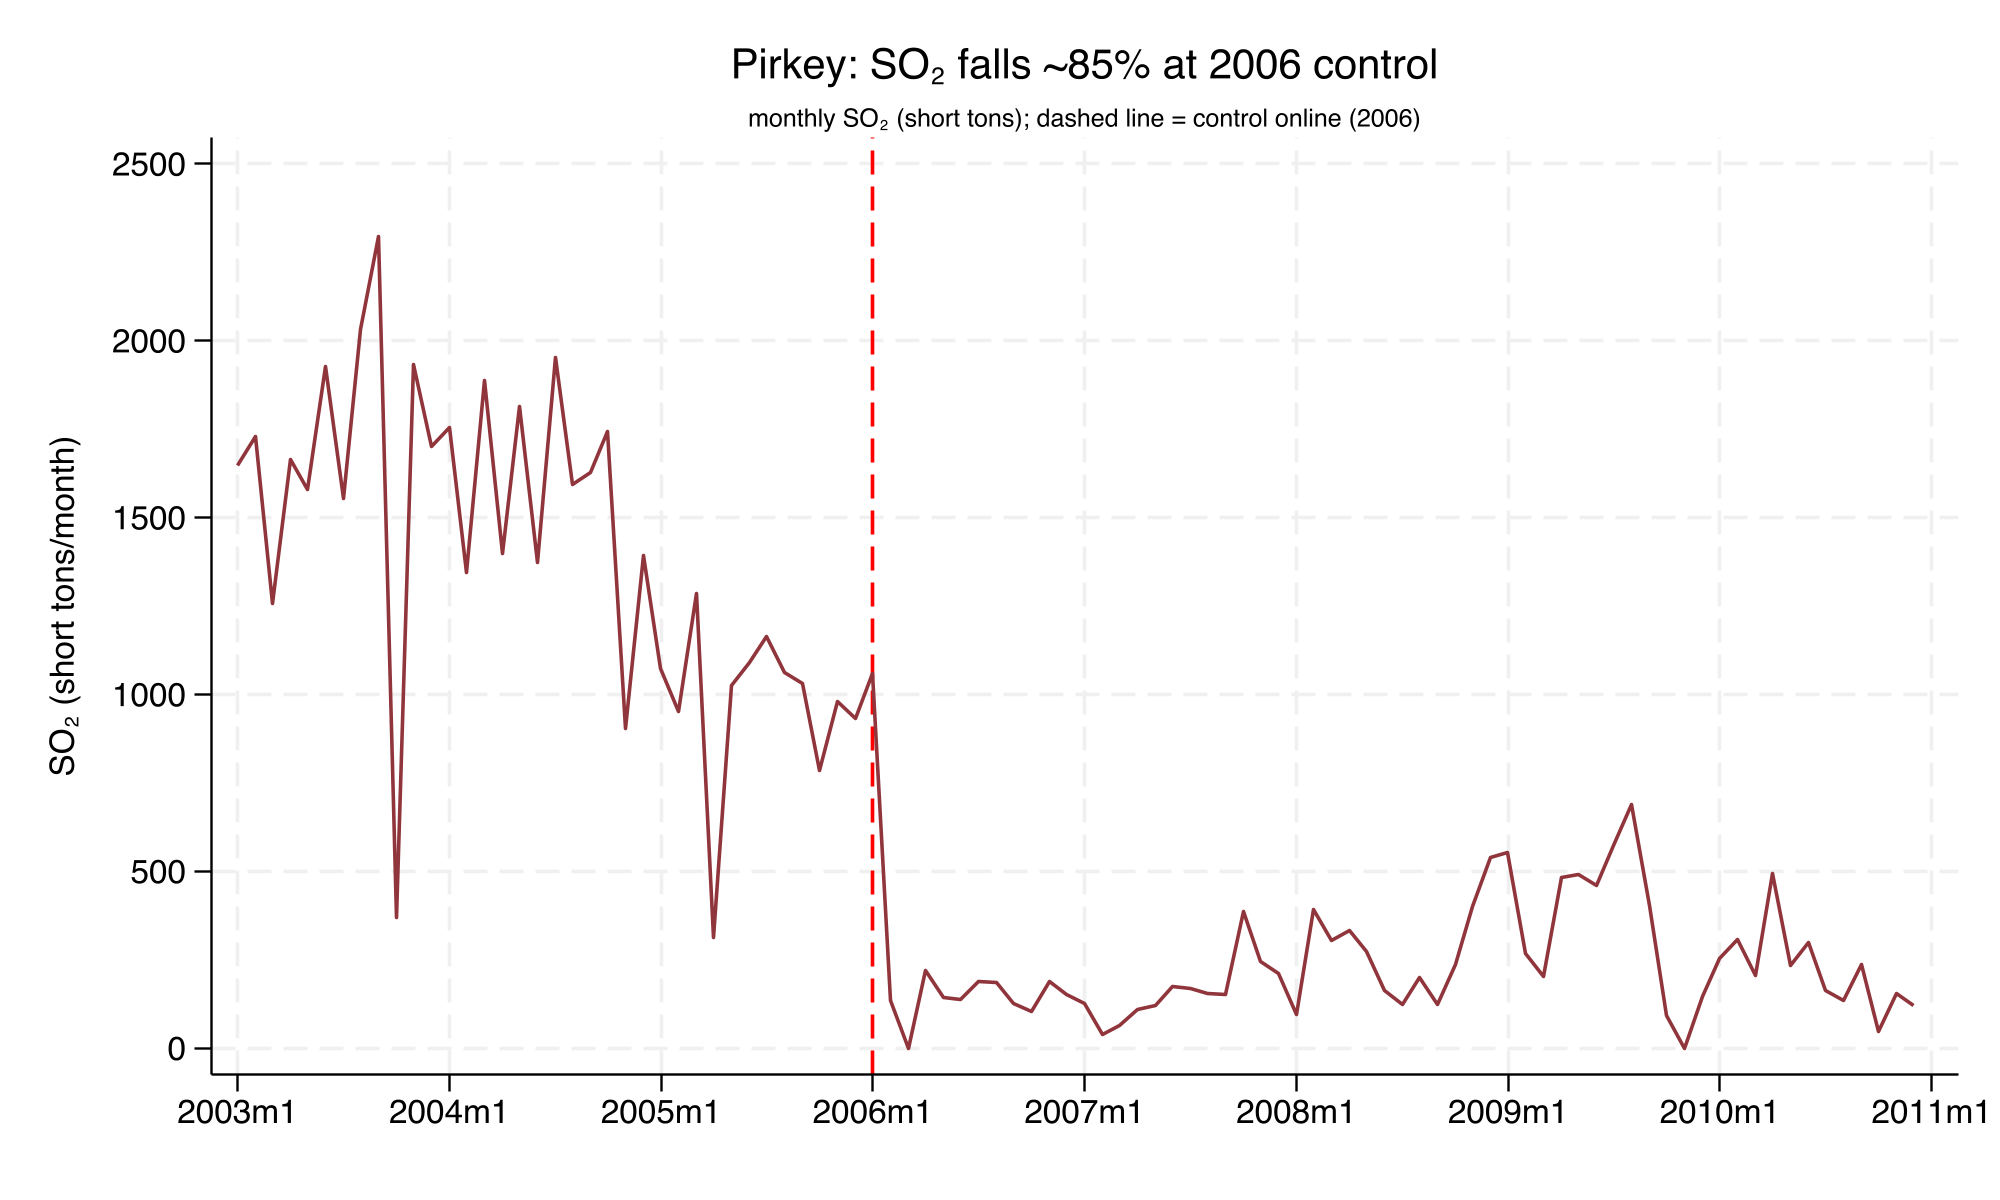
\includegraphics[width=0.49\linewidth]{hero_pirkey_so2.png}
\caption{Link 1, verified: plant emissions fall sharply at control-retrofit dates (EPA CEMS).
Left: W.A.\ Parish NO$_x$ at SCR (2004). Right: Pirkey SO$_2$ at 2006 control.}
\label{fig:firststage}
\end{figure}

\section{Mechanism and Interpretation}
% [DRAFT] The null is informative, not a failure: it localizes where the chain breaks.
Coal SO$_2$/NO$_x$ are precursors to \emph{regional, secondary} particulate matter rather than
\emph{local, primary} exposure at population monitors; ambient SO$_2$ ($\sim$1 ppb) and lead
($\sim$0.01 $\mu$g/m$^3$) were already low in 2005--2010 Texas. Coal's marginal contribution to
local population ambient exposure was therefore too small for retrofit-driven emission changes to
generate detectable infant-health co-benefits in this setting.

\section{Robustness}
% [DRAFT] (i) proximity ITT event study (Callaway--Sant'Anna) on birth weight: ATT $\approx -21$g,
% $p=0.19$, but few (11) plant-area clusters and pre-trend violations; (ii) continuous tract-level
% CEMS exposure: precise null (+5.6g per SD, 95\% CI $[-7,+18]$); (iii) 2SLS unidentified (weak
% instrument). All point the same way.

\section{Conclusion}
% [DRAFT] We provide a CEMS-verified, U.S. estimate of the local infant-health co-benefits of
% coal-plant control retrofits and find them undetectable, with a clear mechanistic explanation.
% Implications for where pollution-control co-benefits should be sought (regional PM, mortality
% margins) and for cost--benefit accounting.

\bibliographystyle{plainnat}
\bibliography{../Bibliography_base}

\end{document}
